\index{Desarrollo|(}
\section{Desarrollo}

En esta secci\'on se explica detalladamente cada uno de los filtros \'utilizados para procesar las im\'agenes:

\subsection{Recortar}
El filtro Recortar \'unicamente requiere copiar una cantidad tam de p\'ixeles de las esquinas de la imagen fuente para generar la imagen destino con las esquinas invertidas.
\subsubsection{Implementaci\'on en C:}
Con dos ciclos anidados se recorre el \'area de tam x tam en cada esquina de la imagen fuente y se escribe en la esquina opuesta de la imagen destino.
\subsubsection{Implementaci\'on en asm}
Tambi\'en se realiza con dos ciclos anidados, pero trayendo de a 16 p\'ixeles por vez.\newline

En cada iteración se traen 16 p\'ixeles de la parte A a xmm0 con la operaci\'on MOVUPS y luego se copian a la parte D, lo mismo con 16 p\'ixeles de B en C, de C en B y de D en A. Esto puede verse en el siguiente gr\'afico.
\begin{center}
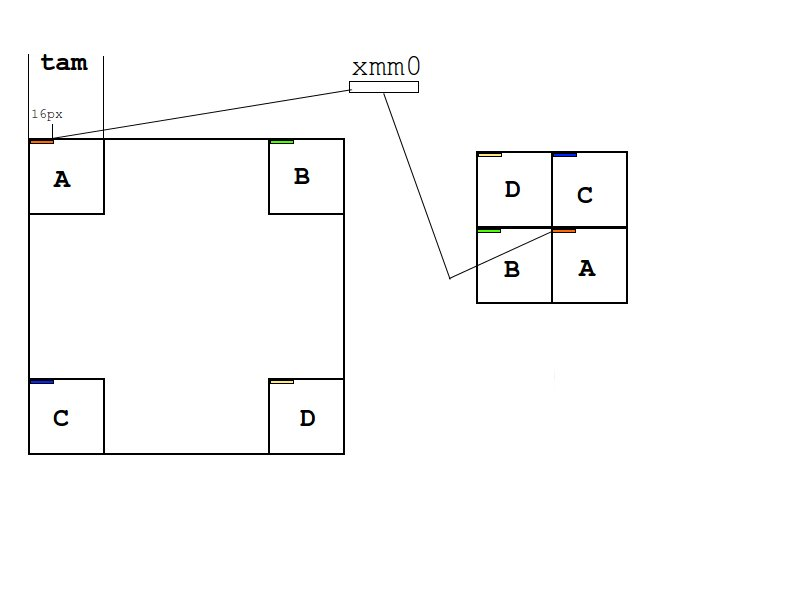
\includegraphics[scale=0.5]{recortar.jpg}
\end{center}
\subsubsection{Resultados}
Dado que en este filtro no se modifican los p\'ixeles, la \'unica diferencia deber\'ia ser en los accesos a memoria. Los ciclos en ambas implementaciones hacen 8 accesos a memoria, 4 lecturas y 4 escrituras, pero la implementaci\'on en ASM accede de a 16 bytes vs 1 de la implementaci\'on en C.\newline
\newline
Por lo tanto la ímplementación en C deber\'ia ser aproximadamente 16 veces m\'as r\'apida.
\begin{center}
	\begin{tabular}{| 1 | 1 | 1 |}
	\hline
	Medici\'on & Implementaci\'on en C & Implementaci\'on en asm \\ \hline
	Ciclos en Total & 422596036 & 24781328 \\  \hline
	Ciclos por llamada & 422596.031 & 24781.328 \\ \hline	
	\end{tabular}
\end{center}

En promedio, cada ejecuci\'on de la implementaci\'on en C tarda 422 596 ciclos y cada ejecuci\'on de ASM 24 781, es decir, ~17 veces m\'as r\'apido, corroborando nuestra hip\'otesis.
\newline

\subsection{Halftone}
El filtro Halftone parte a la imagen original en bloques de 2x2 p\'ixeles, se obtiene t como la sumatoria del valor de cada pixel y genera un bloque del mismo tama\~no en la imagen destino que cumpla:\newline

\begin{center}
	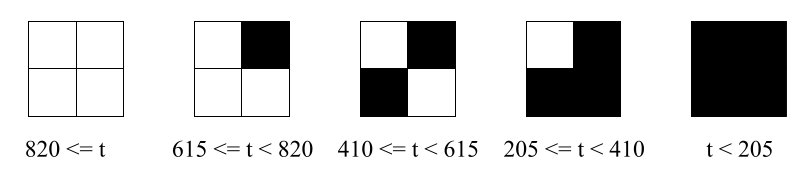
\includegraphics[scale=0.5]{halftone1.jpg}
\end{center}
\newline
Esto implica:\newline
El pixel de arriba a la izquierda es blanco si t $>=$ 205.\newline
El pixel de arriba a la derecha es blanco si t $>=$ 820.\newline
El pixel de abajo a la izquierda es blanco si t $>=$ 615.\newline
El pixel de abajo a la derecha es blanco si t $>=$ 410.\newline
Si el ancho y/o alto de la imagen es impar, se descarta la \'ultima fila y/o columna, seg\'un corresponda.\newline
\subsubsection{Implementaci\'on en C}
\indent Con dos ciclos anidados se recorre de 2 en 2 la imagen original.\newline
Se calcula t con la suma de de los valores de los 4 p\'ixeles y luego se setean los p\'ixeles en blanco o negro seg\'un corresponda por el valor de t.\newline
\subsubsection{Implementaci\'on en asm}
Tambi\'en se realizan dos ciclos alineados, trayendo cada vez de a 32 p\'ixeles. \newline
Se traen 16 p\'ixeles de la primera l\'inea a xmm0 y 16 de la segunda l\'inea a xmm1.\newline
Como para calcular t se necesita un espacio de m\'as de 1 byte (t puede ser mayor a 255), se desempaquetan y se trabaja primero con los 8 bytes menos significativos, guardando el resto.\newline
Se suman los 2 registros verticalmente, luego se shiftea un registro para acomodar y volver a sumar.
Esto da como resultado el valor t para cada uno de los 4 bloques.\newline
\begin{center}
	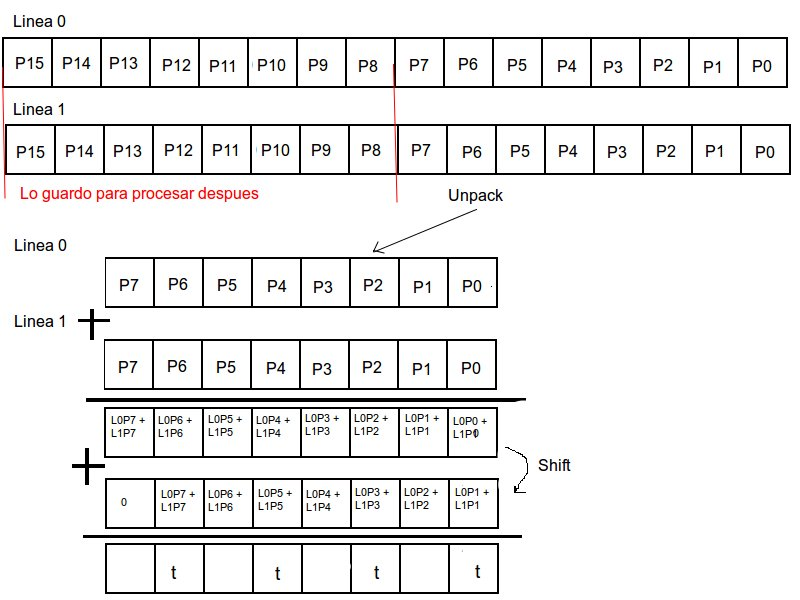
\includegraphics[scale=0.5]{halftone2.jpg}
\end{center}
\newline
Se compara por mayor o igual en un registro distinto para cada uno de los valores l\'imite.\newline
Luego, ya que  el valor que va a cada pixel es el mismo que el resultado de la comparaci\'on (todos 1s o todos 0s), simplemente se ordenan los resultados en los primeros 8 bytes de cada registro.\newline
\begin{center}
	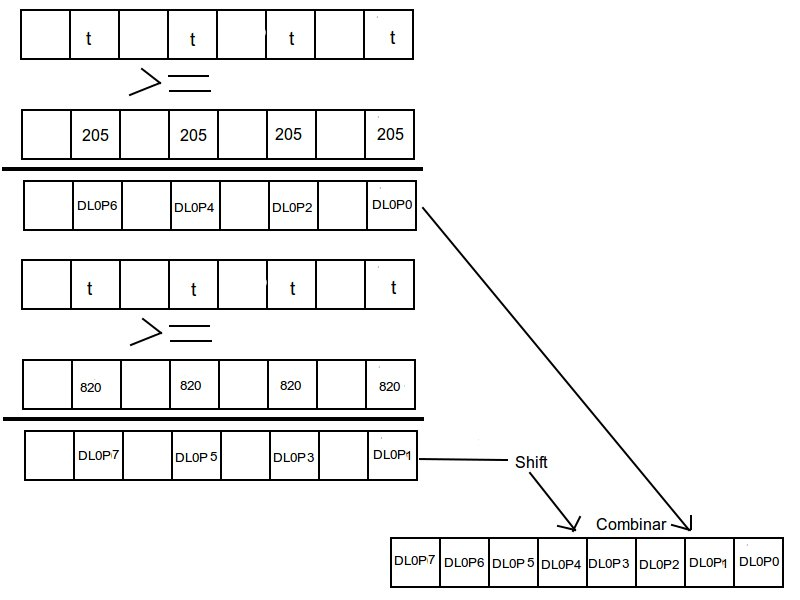
\includegraphics[scale=0.5]{halftone3.jpg}
\end{center}
\newline
Este proceso se repite con los 8 bytes m\'as significativos que guardamos al principio. Estos resultados se shiftean 8 bytes a la izquierda y combinan (con un por) con los primeros resultados, d\'andonos 2 registros con 16 bytes procesados cada uno, que se copian a la memoria de la imagen destino.\newline
\indent 
En el caso que el ancho no sea m\'ultiplo de 16, antes de entrar al ciclo se calcula el resto (width $%$ 16) y en la primera iteraci\'on de cada fila se suma este resto en lugar de los 16 que se suman normalmente.\newline

\subsubsection{Resultados}
En la implementaci\'on en C, para procesar un bloque de 4 p\'ixeles se requieren 8 accesos a memoria (4 lecturas y 4 escrituras), en cambio en la implementaci\'on en ASM, se procesa un bloque de 32 p\'ixeles con tan s\'olo 4 accesos a memoria.\newline
\indent Con esos datos y, teniendo en cuenta que el acceso a memoria es mucho m\'as lenta que cualquier otra operaci\'on que se aplique en el filtro, la implementaci\'on en ASM deber\'ia ser 16 veces m\'s r\'apida que la implementaci\'on en C.\newline

\begin{center}
	\begin{tabular}{| 1 | 1 | 1 |}
	\hline
	Medici\'on & Implementaci\'on en C & Implementaci\'on en asm \\ \hline
	Ciclos en Total & 3229822124 & 230612631 \\  \hline
	Ciclos por llamada & 3229822.250 & 230612.625 \\ \hline	
	\end{tabular}
\end{center}

\indent En promedio, cada ejecuci\'on de la implementaci\'on en C tarda 3 229 822 ciclos y cada ejecuci\'on de ASM tarda 230 612, es decir, ~14 veces más r\'apido, corroborando nuestra hip\'otesis.

\subsection{Rotar}
\indent Este filtro consiste en rotar la imagen 45\° en sentido antihorario. Lo que provoca que algunos pixels se pierdan mientras que otros se anulen (es decir, se vuelvan 0), otros intercambien lugares y por \'ultimo el centro rote sobre si mismo.\newline
\indent Un caso que resulta p\'articular con este filtro y es que su p\'erformance casi no var\'ia respecto de assembler o C. Esto sucede porque hay que tratar cada pixel (o byte si nos referimos al c\'odigo) de manera p\'articular, haciendo que no sea posible paralelizar tanto como sucede con otros filtros.

\subsubsection{Algoritmo}
\begin{enumerate}
\item Crear las variables/Registros para almacenar los datos y las constantes a utilizar.
\item Loop:
	\begin{enumerate}
	\item Crear los respectivos u y v que se calculan dependiendo de la posicion de mi pixel de entrada.\newline
	u = c_x + \frac{\sqrt{2}}{2}(x - c_x) - \frac{\sqrt{2}}{2}(y - c_y)\newline
	v = c_y + \frac{\sqrt{2}}{2}(x - c_x) - \frac{\sqrt{2}}{2}(y - c_y)\newline
	c_x = [I_{src\_width}/2]\newline
	c_y = $ [I_{src\_height}/2]$\newline	
	\item Analizo si u y v cumplen los requisitos de para realizar el intercambio de pixels.\newline
	$0 <= u < I_{src\_width} $ y $ 0 <= v < I_{src\_height}$\newline
	\item Si lo cumple entonces el nuevo valor de $I_{dst}[x][y] = I_{src}[u][v]$.\newline
	\item De lo contrario, 	I_{dst}[x][y] = $0$. \footnote{ver codigo de la implementaci\'on para un mejor entendimiento.}\newline
	
	\end{enumerate}
	\item Finalmente devuelve a matriz rotada.
\end{enumerate}

\subsubsection{Resultado}
\indent Como resultado de este filtro remarcamos la poca diferencia entre C y assembler con respecto a lo que sucede en los dem\'as filtros. Como datos, sabemos que:\newline
\newline
\begin{tabular}{| 1 | 1 |}
\hline
Medici\'on & Implementaci\'on en C \\ \hline
Ciclos Totales & 1645260830 \\ \hline
Ciclos Por Llamada & 16452608.000 \\ \hline

\end{tabular}
\index{Desarrollo|)}